\documentclass[11pt, a4paper]{article}

% --- 基本頁面設定 ---
\usepackage[a4paper, top=2.5cm, bottom=2.5cm, left=2cm, right=2cm]{geometry}

% --- 圖片處理與定位套件 (新增與修正) ---
\usepackage{graphicx} 
\usepackage{float}    % 必須載入此套件才能使用 [H] 選項

% --- XeLaTeX 專用中文套件 ---
% 使用這個套件在 Windows 上跑 XeLaTeX 是最穩定的
\usepackage{xeCJK}

% 設定中文字體：微軟正黑體 (Windows 內建)
\setCJKmainfont{Microsoft JhengHei}

% 設定英文字體：Arial (Windows 內建)
\setmainfont{Arial}

% --- 數學與表格套件 ---
\usepackage{amsmath}
\usepackage{booktabs}
\usepackage{enumitem}
\setlist[itemize]{label=-}
\usepackage{multicol}

% --- 1. Title (標題) ---
\title{\textbf{Implementation of Matrix Calculus and Numerical Differentiation for Deep Learning Foundations in Java}}

% --- 個人資訊 ---
\author{蔡晟旭 \\ 
Student ID: 1113405013 \\
國立澎湖科技大學 資訊工程學系 \\
National Penghu University of Science and Technology}
\date{\today}

\begin{document}

\maketitle

% --- 2. Abstract (摘要) ---
\begin{abstract}
本報告探討深度學習中不可或缺的兩項數學基石：矩陣運算與數值微分。透過 Java 語言實作矩陣乘法演算法與基於中心差分法（Central Difference Method）的導數計算。實驗旨在驗證數值逼近的準確性，並探討步長 $h$ 對微分誤差的影響。所有原始碼均符合不使用進階內建套件之規範，並託管於 GitHub。
\\ \\
% --- 3. GitHub 網址 ---
\textbf{GitHub Repository:} https://github.com/tch107146/JAVA-0303-Assignments-3
\end{abstract}

% --- 4. Keywords (關鍵字) ---
\noindent \textbf{Keywords:} Matrix Multiplication, Numerical Differentiation, Taylor Expansion, Java, Deep Learning Foundations.

\begin{multicols}{2}

% --- 5. Introduction (引言) ---
\section{Introduction}
神經網路的運作本質上是大量的線性代數與梯度下降運算。本實驗（Assignment 3）透過程式實作這些底層邏輯，不僅加深了對矩陣維度變化的理解，也透過數值微分模擬了神經網路中反向傳播獲取梯度的核心過程。

% --- 6. Methodology (研究方法) ---
\section{Methodology}
\subsection{Matrix Multiplication}
設 $A$ 為 $m \times n$ 矩陣，$B$ 為 $n \times p$ 矩陣，其乘積 $C$ 之定義為：
\begin{equation}
C_{ij} = \sum_{k=0}^{n-1} A_{ik} B_{kj}
\end{equation}

\subsection{Numerical Derivative}
根據泰勒展開式，函數 $f(x)$ 在 $x$ 點的導數可由中心差分法近似：
\begin{equation}
f'(x) \approx \frac{f(x+h) - f(x-h)}{2h}
\end{equation}
本實驗針對 $f(x) = x^2$ 進行測試，理論解為 $f'(x) = 2x$。

% --- 7. Implementation Details (實作細節) ---
\section{Implementation Details}
\begin{itemize}
    \item \textbf{Matrix Computation}: 透過三層嵌套 \texttt{for} 迴圈實作，並定義 \texttt{MatrixMath} 類別。
    \item \textbf{Calculus Simulation}: 定義 \texttt{CalculusMath} 類別，封裝函數定義與差分公式。
    \item \textbf{Precision}: 使用 \texttt{double} 型別以確保浮點運算的精確度。
\end{itemize}

% --- 8. Experimental Results (實驗結果) ---
\section{Experimental Results}
經測試矩陣乘法，結果符合預期。針對導數部分，設定 $x=2$，$h=0.0001$，程式計算結果高度逼近理論值 4.0。

% --- 圖片插入部分 ---
\begin{figure}[H] % 使用 [H] 強制固定圖片在文字中間
  \centering
  % 使用 IfFileExists 檢查圖片，防止報錯卡住編譯
  \IfFileExists{screenshot.png}{
    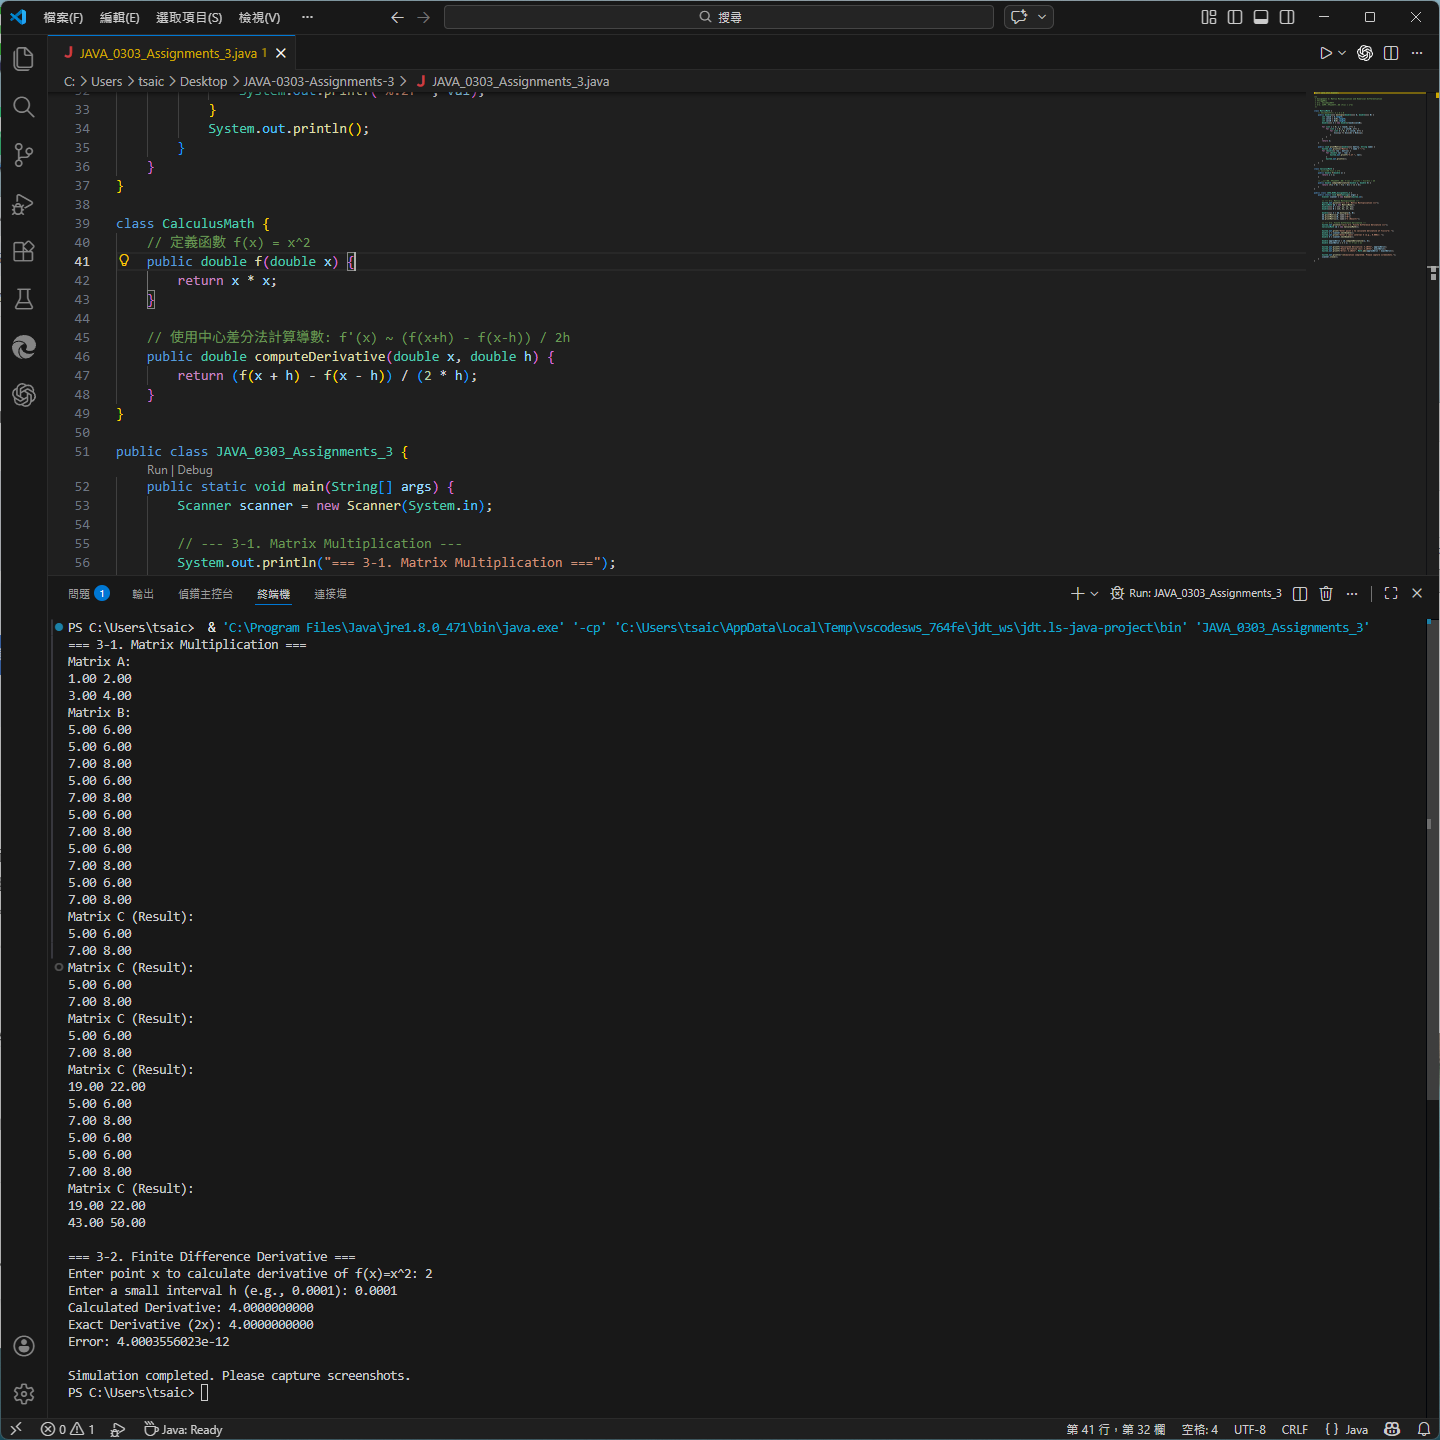
\includegraphics[width=0.9\columnwidth]{screenshot.png}
  }{
    \framebox{\parbox{0.8\columnwidth}{\centering \vspace{1.2cm} \textbf{[ 圖片截圖提示 ]} \\ 請將 Java 執行截圖命名為 \\ \texttt{screenshot.png} \\ 並放在本 .tex 檔同目錄 \vspace{1.2cm}}}
  }
  \caption{Execution output of matrix and derivative computation.}
  \label{fig:result}
\end{figure}

% --- 9. Discussion (討論) ---
\section{Discussion}
實驗顯示步長 $h$ 的選擇極為關鍵。雖然理論上 $h$ 愈小愈精確，但在程式實作中，過小的 $h$ 可能引發浮點數捨入誤差。中心差分法相較於前向差分法具有較高的二階精度。

% --- 10. Conclusion (結論) ---
\section{Conclusion}
本作業完成了深度學習基礎運算的實作，強化了對線性代數維度匹配與數值分析誤差來源的認識，為後續開發複雜的神經網路架構奠定了基礎。

% --- 11. References (參考文獻) ---
\section{References}
\noindent [1] H. Rui, \textit{Lecture 0: Preliminary Introduction}, NPU, 2025. \par
\noindent [2] I. Goodfellow, Y. Bengio, and A. Courville, \textit{Deep Learning}, MIT Press, 2016.

\end{multicols}

\end{document}